\documentclass[11pt]{article}
\usepackage[margin=1in]{geometry}
\usepackage{amsmath,amssymb,amsthm,mathtools}
\usepackage{graphicx}
\usepackage{microtype}
\usepackage[hidelinks]{hyperref}
\usepackage{enumitem}

\newtheorem{theorem}{Theorem}
\newtheorem{lemma}{Lemma}
\newcommand{\Spp}{\mathbb S_{++}}
\newcommand{\diag}{\operatorname{diag}}
\newcommand{\tr}{\operatorname{tr}}
\newcommand{\E}{\mathbb E}
\newcommand{\Pp}{\mathbb P}

\title{One-factor association of disjoint principal minors\\
of Wishart random matrices}
\author{Candidate partial result for arXiv:2311.00202\\
\texttt{agent\_lane\_09}, model GPT5.6}
\date{22 July 2026}

\begin{document}
\maketitle

\begin{center}
\fbox{\parbox{0.91\linewidth}{\textbf{Status.}
\texttt{partial\_result\_likely\_valid; human\_review\_needed}.
The unrestricted conjectures remain open.}}
\end{center}

\section{Source questions}

Genest, Ouimet, and Richards~\cite{GOR} consider
\(\mathfrak X\sim\mathcal W_p(\alpha,\Sigma)\), with
\(\alpha>p-1\), partitioned into diagonal blocks
\(\mathfrak X_{ii}\) of sizes \(p_i\), where \(\sum_i p_i=p\).
Their Conjecture~1.1 asks whether, for every \(\nu_i\geq0\),
\begin{equation}\label{eq:moment-source}
 \E\prod_{i=1}^d|\mathfrak X_{ii}|^{\nu_i}
 \ \geq\ \prod_{i=1}^d\E|\mathfrak X_{ii}|^{\nu_i}.
\end{equation}
The statement is on source page 5:

\begin{center}

\includegraphics[width=\linewidth]{figures/open_problem_crop.png}
\end{center}

Their Conjecture~3.8 asks, for \(2\leq k\leq d\) and \(t_i>0\),
\begin{equation}\label{eq:threshold-source}
\Pp\!\left(\bigcap_{i=1}^d\{|\mathfrak X_{ii}|\leq t_i\}\right)
\geq
\Pp\!\left(\bigcap_{i<k}\{|\mathfrak X_{ii}|\leq t_i\}\right)
\Pp\!\left(\bigcap_{i\geq k}\{|\mathfrak X_{ii}|\leq t_i\}\right).
\end{equation}
The statement crosses source pages 9--10:

\begin{center}
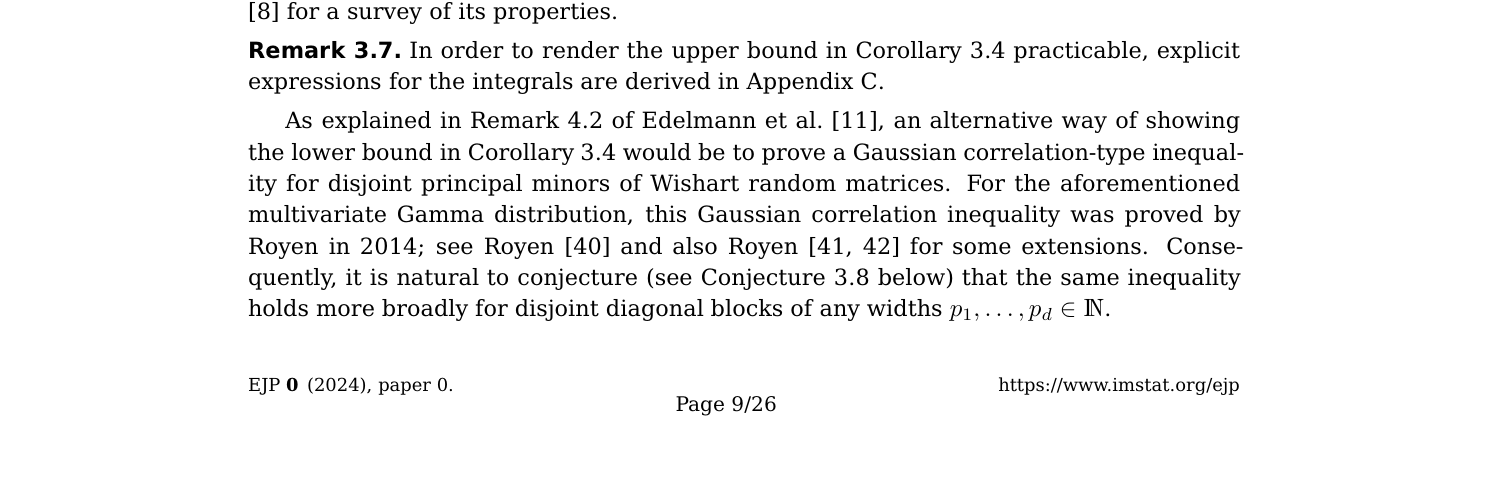
\includegraphics[width=\linewidth]{figures/threshold_conjecture_crop_page9.png}
\smallskip
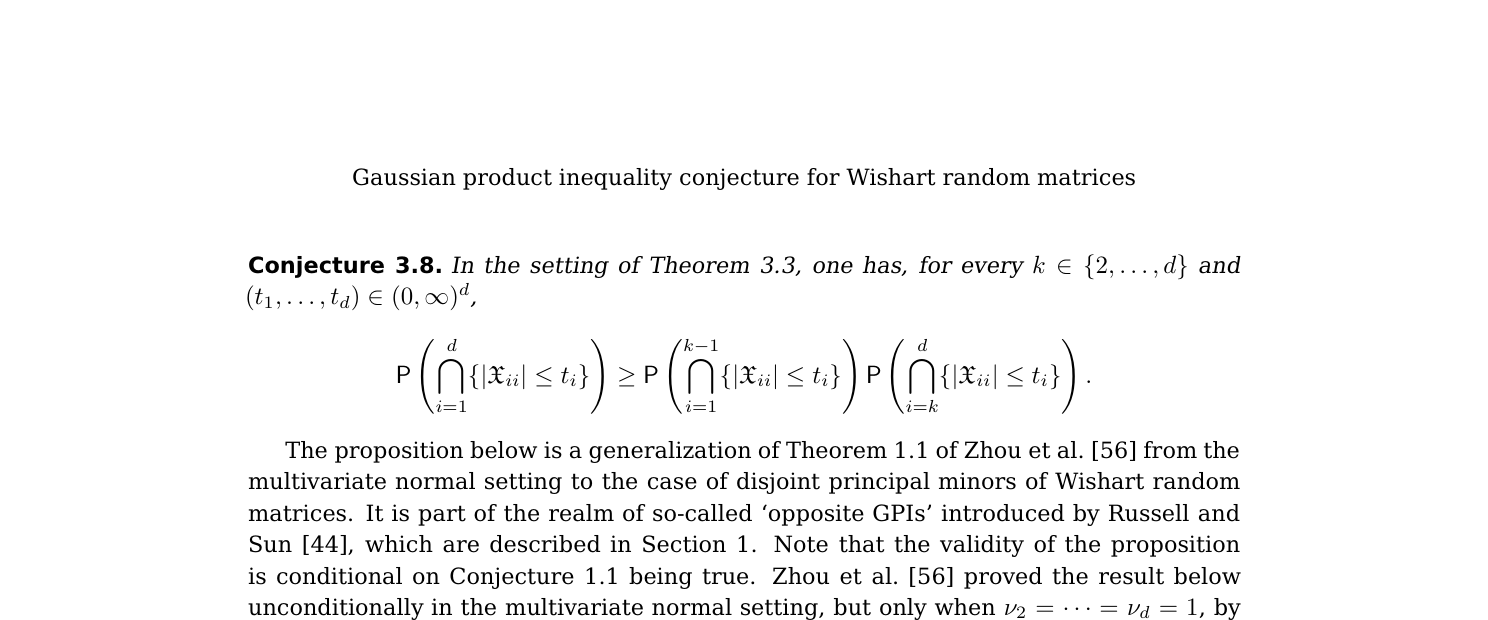
\includegraphics[width=\linewidth]{figures/threshold_conjecture_crop_page10.png}
\end{center}

\section{Result and proof intuition}

Write \(D=\diag(D_1,\ldots,D_d)\), with
\(D_i\in\Spp^{p_i}\), and write \(a=(a_1^\mathsf T,\ldots,
a_d^\mathsf T)^\mathsf T\).  The scale matrices
\begin{equation}\label{eq:factor}
 \Sigma=D+aa^\mathsf T
\end{equation}
are precisely coherent one-factor perturbations of block independence:
\(\Sigma_{ij}=a_i a_j^\mathsf T\) for \(i\neq j\).

\paragraph{Proof intuition.}
For block-diagonal Laplace variables, the matrix determinant lemma separates
the Wishart transform into independent central-block factors and one scalar
factor.  The latter is the Laplace transform of a common
\(\chi^2_\alpha\) variable \(S\).  Conditional on \(S=s\), the blocks are
independent rank-one noncentral Wisharts.  A Schur-complement factorization
then writes each block determinant as a fixed positive random factor times a
noncentral chi-square whose noncentrality is proportional to \(s\).  Thus
conditional positive moments increase with \(s\), whereas conditional lower
tails decrease with \(s\).  Products on either side of any split are monotone
in the same scalar, and the desired inequalities are Chebyshev covariance
inequalities.  What remains open is the several-factor case, where the common
mixing parameter becomes matrix-valued and this total order disappears.

\begin{theorem}[One-factor product association]\label{thm:main}
Let \(p_1,\ldots,p_d\geq1\), \(p=\sum_i p_i\), and
\(\alpha>p-1\).  Suppose \(\Sigma\) has the form \eqref{eq:factor}, and let
\(\mathfrak X\sim\mathcal W_p(\alpha,\Sigma)\), partitioned conformally.
Put \(\Delta_i=|\mathfrak X_{ii}|\).

Let \(h_i:(0,\infty)\to[0,\infty)\) be Borel functions whose required
expectations are finite.  If all \(h_i\) are nondecreasing, or all are
nonincreasing, then for every split \(A\sqcup B=\{1,\ldots,d\}\),
\begin{equation}\label{eq:split}
 \E\prod_{i=1}^d h_i(\Delta_i)
 \ \geq\
 \E\prod_{i\in A}h_i(\Delta_i)\,
 \E\prod_{i\in B}h_i(\Delta_i).
\end{equation}
Consequently \eqref{eq:moment-source} holds for all real \(\nu_i\geq0\),
and \eqref{eq:threshold-source} holds for all \(t_i>0\).
\end{theorem}

\section{Proof}

We use the Wishart convention of~\cite{GOR,Muirhead}:
\begin{equation}\label{eq:central-LT}
 \E\,e^{-\tr(T\mathfrak X)}
 =|I+2T\Sigma|^{-\alpha/2},\qquad T\geq0.
\end{equation}

\subsection{An exact common-scalar mixture}

Take \(T=\diag(T_1,\ldots,T_d)\), \(T_i\geq0\), and set
\[
 q_i(T_i)=
 a_i^\mathsf T T_i(I+2D_iT_i)^{-1}a_i\geq0.
\]
The matrix determinant lemma and the push-through identity give
\begin{align}
 |I+2T(D+aa^\mathsf T)|
 &=
 \prod_{i=1}^d|I+2T_iD_i|
 \left(1+2\sum_{i=1}^d q_i(T_i)\right).\label{eq:detlemma}
\end{align}
Let \(S\sim\chi^2_\alpha\).  Conditional on \(S=s\), let
\(\mathfrak Y_1,\ldots,\mathfrak Y_d\) be independent noncentral Wishart
matrices whose transforms are
\begin{equation}\label{eq:conditional-LT}
 \E\!\left[e^{-\tr(T_i\mathfrak Y_i)}\mid S=s\right]
 =
 |I+2T_iD_i|^{-\alpha/2}e^{-s q_i(T_i)}.
\end{equation}
These laws exist because \(\alpha>p-1\geq p_i-1\); after whitening their
noncentrality matrices are
\(sD_i^{-1/2}a_i a_i^\mathsf T D_i^{-1/2}\), of rank at most one.
Since
\[
 \E e^{-uS}=(1+2u)^{-\alpha/2},
\]
averaging the product of \eqref{eq:conditional-LT} and using
\eqref{eq:detlemma} yields \eqref{eq:central-LT} for every block-diagonal
\(T\).  Uniqueness of Laplace transforms on products of positive-definite
cones gives
\begin{equation}\label{eq:mixture-law}
 (\mathfrak X_{11},\ldots,\mathfrak X_{dd})
 \ \stackrel d=\
 (\mathfrak Y_1,\ldots,\mathfrak Y_d).
\end{equation}
This is valid for every real \(\alpha>p-1\), not only integer degrees of
freedom.

\subsection{Rank-one determinant monotonicity}

\begin{lemma}\label{lem:rankone}
Let \(r\geq1\), \(\beta>r-1\), and let \(Y_\lambda\) be a noncentral
Wishart matrix with degrees of freedom \(\beta\), scale \(I_r\), and
noncentrality \(\lambda e_1e_1^\mathsf T\).  There are independent random
variables
\[
 Q_\lambda\sim\chi'^2_\beta(\lambda),
 \qquad C\sim\mathcal W_{r-1}(\beta-1,I_{r-1}),
\]
with \(|C|=1\) when \(r=1\), such that
\begin{equation}\label{eq:Bartlett}
 |Y_\lambda|\ \stackrel d=\ Q_\lambda |C|.
\end{equation}
In particular \(|Y_\lambda|\) is stochastically nondecreasing in
\(\lambda\).
\end{lemma}

\begin{proof}
The rank-one noncentral Wishart density is the central density multiplied by
\[
 e^{-\lambda/2}\,
 {}_0F_1\!\left(;\frac{\beta}{2};\frac{\lambda y_{11}}{4}\right).
\]
Indeed the matrix hypergeometric series reduces to the scalar series because
the argument has rank one; this is the standard noncentral Wishart density
formula~\cite{Muirhead}.

Under the central law, write
\[
 Y=\begin{pmatrix}x&z^\mathsf T\\z&C+zz^\mathsf T/x\end{pmatrix}.
\]
Then \(|Y|=x|C|\).  The change of variables \(z=\sqrt{x}\,u\) factors the
central density into the densities of
\[
 x\sim\chi^2_\beta,\qquad
 u\sim N_{r-1}(0,I),\qquad
 C\sim\mathcal W_{r-1}(\beta-1,I),
\]
independently.  The noncentral density multiplier depends only on \(x\) and
is exactly the likelihood ratio of \(\chi'^2_\beta(\lambda)\) relative to
\(\chi^2_\beta\).  It therefore replaces \(x\) by \(Q_\lambda\) without
changing the independent law of \(C\), proving \eqref{eq:Bartlett}.

Finally, if \(N_\lambda\sim\operatorname{Poisson}(\lambda/2)\), then
\[
 Q_\lambda\mid N_\lambda\sim\chi^2_{\beta+2N_\lambda}.
\]
For \(\lambda'\geq\lambda\), couple
\(N_{\lambda'}=N_\lambda+\widetilde N\) with an independent
\(\widetilde N\sim\operatorname{Poisson}((\lambda'-\lambda)/2)\), and add
independent chi-squares of two degrees of freedom.  This couples
\(Q_{\lambda'}\geq Q_\lambda\), hence also
\(Q_{\lambda'}|C|\geq Q_\lambda|C|\).
\end{proof}

For block \(i\), whiten by \(D_i^{-1/2}\) and rotate
\(D_i^{-1/2}a_i\) to the first coordinate.  Lemma~\ref{lem:rankone} and
\eqref{eq:conditional-LT} show that, conditional on \(S=s\),
\begin{equation}\label{eq:blockfactor}
 |\mathfrak Y_i|
 \ \stackrel d=\
 |D_i|\,Q_{i,s}B_i,\qquad
 Q_{i,s}\sim
 \chi'^2_\alpha\!\left(s\,a_i^\mathsf T D_i^{-1}a_i\right),
\end{equation}
where \(B_i>0\) has a law independent of \(s\) and is independent of
\(Q_{i,s}\).  Hence the conditional law of \(|\mathfrak Y_i|\) is
stochastically nondecreasing in \(s\).

\subsection{Scalar association}

Set
\[
 m_i(s)=\E[h_i(|\mathfrak Y_i|)\mid S=s].
\]
By \eqref{eq:blockfactor}, all \(m_i\) are nondecreasing when all \(h_i\)
are nondecreasing, and all are nonincreasing when all \(h_i\) are
nonincreasing.  Conditional independence and \eqref{eq:mixture-law} give
\[
 \E\prod_{i=1}^d h_i(\Delta_i)
 =\E\prod_{i=1}^d m_i(S).
\]
Put \(M_A=\prod_{i\in A}m_i\) and \(M_B=\prod_{i\in B}m_i\).  These two
functions have the same monotonicity direction.  If \(S'\) is an independent
copy of \(S\), Chebyshev's covariance identity gives
\[
 \operatorname{Cov}(M_A(S),M_B(S))
 =\frac12\E\!\left[
 (M_A(S)-M_A(S'))(M_B(S)-M_B(S'))\right]\geq0.
\]
This is precisely \eqref{eq:split}.

Taking \(h_i(x)=x^{\nu_i}\) and iterating splits proves
\eqref{eq:moment-source}.  Taking
\(h_i(x)=\mathbf1_{\{x\leq t_i\}}\) and the split
\(A=\{1,\ldots,k-1\}\), \(B=\{k,\ldots,d\}\) proves
\eqref{eq:threshold-source}. \qed

\section{Verification and limitations}

\begin{itemize}[leftmargin=*]
\item The proof was checked separately at the three structural points:
the determinant-lemma transform, the rank-one density tilt, and the scalar
covariance step.
\item The accompanying program compares direct SciPy Wishart samples with
the determinant mixture for randomized noninteger degrees of freedom, and
tests both inequalities.  This is a smoke test, not part of the proof.
\item The result includes arbitrary block sizes, arbitrary \(d\), every
real \(\alpha>p-1\), every real \(\nu_i\geq0\), and every \(t_i>0\).
\item It does not settle a general \(\Sigma\).  With several latent factors,
the conditional noncentrality is governed by a matrix Gram parameter; varying
one latent factor can change cross terms in both directions, so the scalar
stochastic-order argument does not iterate.
\end{itemize}

\paragraph{Novelty check.}
The four local run indexes had no hit for arXiv:2311.00202 or this route.
Bounded searches covered the exact conjecture labels, source title,
\emph{one-factor Wishart Gaussian product inequality},
\emph{rank-one noncentral Wishart determinant stochastic monotonicity}, and
papers citing the source.  The two-block theorem of~\cite{GORtwo} and the
July 2026 finite Stein recursion of~\cite{GO} were inspected.  No statement
of Theorem~\ref{thm:main} was found.  Novelty is therefore plausible, not
certified.

\paragraph{Human-review recommendation.}
Verify especially the noncentral-Wishart parameter convention in
\eqref{eq:conditional-LT}, the rank-one density reduction in
Lemma~\ref{lem:rankone}, and Laplace-transform uniqueness for the joint
diagonal-block law.  If those pass, retain this as a substantial partial
answer to both source conjectures.

\begin{thebibliography}{9}
\bibitem{GOR}
C. Genest, F. Ouimet, and D. Richards,
\emph{On the Gaussian product inequality conjecture for disjoint principal
minors of Wishart random matrices},
Electron. J. Probab. 29 (2024), arXiv:2311.00202v3,
doi:10.1214/24-EJP1222.

\bibitem{GORtwo}
C. Genest, F. Ouimet, and D. Richards,
\emph{An explicit Wishart moment formula for the product of two disjoint
principal minors},
Proc. Amer. Math. Soc. 153 (2025), 1299--1311,
arXiv:2409.14512.

\bibitem{GO}
R. E. Gaunt and F. Ouimet,
\emph{On Wilks' problem: Exact recursive formulas via Stein's method for the
joint moments of disjoint principal minors of Wishart random matrices},
arXiv:2607.03984v1 (2026).

\bibitem{Muirhead}
R. J. Muirhead,
\emph{Aspects of Multivariate Statistical Theory},
Wiley, 1982.
\end{thebibliography}

\end{document}
